\documentclass[tikz,border=3mm]{standalone}
\begin{document}

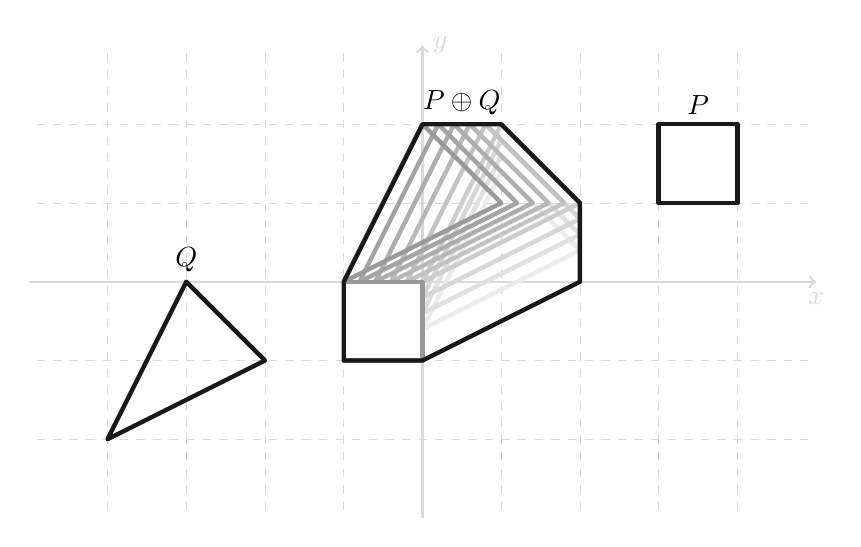
\begin{tikzpicture}
  % axes
  \draw[help lines, color=gray!30, dashed] (-4.9,-2.9) grid (4.9,2.9);
  \draw[->, thick, color=gray!30] (-5,0)--(5,0) node[below]{$x$};
  \draw[->, thick, color=gray!30] (0,-3)--(0,3) node[right]{$y$};

  % p
  \draw[ultra thick, color=black!90, line join=round] (3,1) -- (4,1) -- (4,2) -- (3,2) -- cycle;
  \draw (3.5,2) node[above]{$P$};

  % q
  \draw[ultra thick, color=black!90, line join=round] (-4,-2) -- (-3,0) -- (-2,-1) -- cycle;
  \draw (-3,0) node[above]{$Q$};

  % p + q shades
  \draw[ultra thick, color=black!4, line join=round] (0,-.2) -- (1,1.8) -- (2,.8) -- cycle;
  \draw[ultra thick, color=black!8, line join=round] (0,-.6) -- (1,1.4) -- (2,.4) -- cycle;
  \draw[ultra thick, color=black!12, line join=round] (0,-.4) -- (1,1.6) -- (2,.6) -- cycle;
  \draw[ultra thick, color=black!16, line join=round] (0,-.2) -- (1,1.8) -- (2,.8) -- cycle;
  \draw[ultra thick, color=black!20, line join=round] (0,0) -- (1,2) -- (2,1) -- cycle;
  \draw[ultra thick, color=black!24, line join=round] (-.2,0) -- (0.8,2) -- (1.8,1) -- cycle;
  \draw[ultra thick, color=black!28, line join=round] (-.4,0) -- (0.6,2) -- (1.6,1) -- cycle;
  \draw[ultra thick, color=black!32, line join=round] (-.6,0) -- (0.4,2) -- (1.4,1) -- cycle;
  \draw[ultra thick, color=black!36, line join=round] (-.8,0) -- (0.2,2) -- (1.2,1) -- cycle;
  \draw[ultra thick, color=black!40, line join=round] (-1,0) -- (0,2) -- (1,1) -- cycle;
  \draw[ultra thick, color=black!40, line join=round] (-1,-1) -- (0,-1) -- (0,0) -- (-1,0) -- cycle;



  % p + q
  \draw[ultra thick, color=black!90, line join=round] (0,2) -- (1,2) -- (2,1) -- (2,0) -- (0,-1) -- (-1,-1) -- (-1,0) -- cycle;
  \draw (0.5,2) node[above]{$P \oplus Q$};
  
\end{tikzpicture}

\end{document}